343. \begin{figure}[ht!]
\center{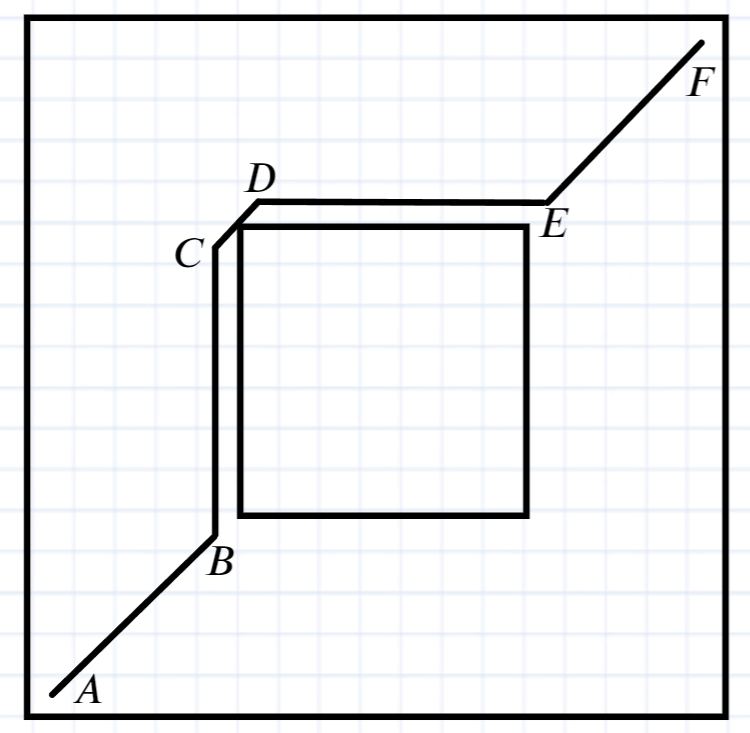
\includegraphics[scale=0.35]{murav.png}}
\end{figure}\\
Чтобы добраться из точки $A$ до точки $B$ и из точки $E$ до точки $F,$ жуку надо сделать по $(2025-7):2-1=1008$ шагов. Чтобы добраться от точки $B$ до точки $C$ и от точки $D$ до точки $E$ ему понадобится по 7 шагов. Чтобы добраться от точки $C$ до точки $D$ ему понадобится 1 шаг. Значит, всего ему надо сделать $1008\cdot2+7\cdot2+1=2031$ шаг.\\
